\chapter{Robert Miller: Reputation, Cashflow, and the Cost of Value}

Robert Miller's interview begins with a compact paradox: the first company can close, the second company can close, and yet something built alongside them can keep working. In this conversation that durable thing is not a machine, a patent, or a balance-sheet asset. It is personal brand, reputation, accumulated skill, and the market's memory that a person can produce results. We will keep the numerical claims in their spoken form, treat the mechanisms as interview claims, and use a small amount of notation only to make the commercial logic visible.

\section{From Capital Gains to Cashflow}

The opening teaser starts in the middle of the story. Robert says that with his first agency he was also building a personal brand. That agency shut down. A second agency also shut down. Then the third business, in his account, scaled to multiple seven figures within about six months because the personal brand had already been built. A newer business was already at a seven-figure runway within roughly sixty days.

The formal interview then backs up and gives us the origin: digital marketing, e-commerce, and crypto, all entered early. Robert says he was in the crypto space from age seventeen or eighteen, with 2015--2016 as the approximate starting window. The important distinction comes when he talks about having made money in crypto before taking a digital marketing course. That money was not yet a business.

\begin{equation}
\hbox{capital gains} \neq \hbox{cashflow}.
\end{equation}

This is the first real hinge in the interview. A gain from an appreciating asset may create capital, but it does not by itself create an operating engine. The simpler bookkeeping identity is plain:

\begin{equation}
\hbox{cashflow} = \hbox{cash in} - \hbox{cash out}.
\end{equation}

Robert's point is not that capital gains are useless. Quite the opposite: the early crypto gain gave him capital, attention, and confidence. But he treats it as incomplete until it is converted into skill, service, sales, and repeatable business motion.

\subsection{Question \& Answer}

\paragraph{Question.} Why were crypto gains not enough?

\paragraph{Answer.} Because, in Robert's framing, they were capital gains rather than cashflow. A crypto position can rise; a person can make money from that rise; but a business requires a way to repeatedly create demand, make sales, deliver value, and understand where the cash is going. This is why the story pivots from crypto to digital marketing. He needed to learn how to build a real business, not merely hold an asset that had gone up.

\section{Scaling as Marketing, Sales, and Finance}

Once the interview asks about scaling a business, Robert gives a three-part stack. First comes marketing: not merely paid advertising, but content, traffic, and getting people to care about what one says and does. He names Facebook, TikTok, Instagram, and YouTube as examples of attention channels.

Second comes sales. If a person is weak at sales but has many leads, something may still happen. If a person is strong at both marketing and sales, Robert says growth can happen quickly. Third comes the less glamorous item: finance, meaning the understanding of cashflows.

A cautious reconstruction of his operating model is:

\begin{equation}
R \approx L \cdot c \cdot P,
\end{equation}

where \(R\) denotes revenue, \(L\) denotes leads or traffic, \(c\) denotes the conversion or close rate, and \(P\) denotes average purchase or contract value. Robert does not write this equation; it is our compact way to represent the sequence he speaks: attention creates leads, sales converts leads, and finance determines whether the resulting revenue actually strengthens the business.

\begin{figure}
\centering
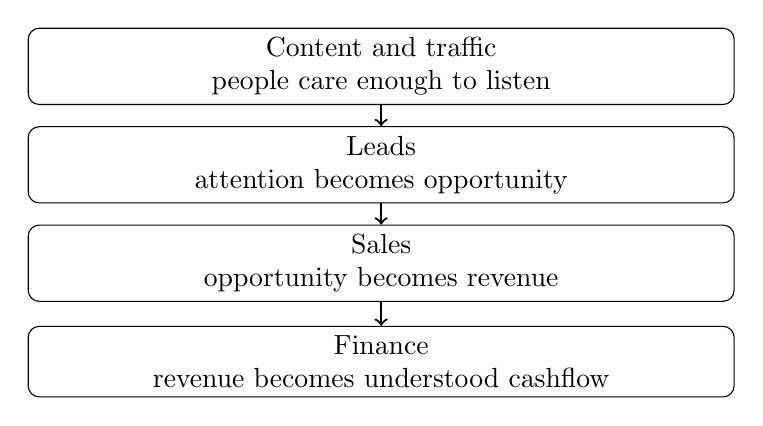
\begin{tikzpicture}[
  box/.style={draw, rounded corners, align=center, text width=0.72\linewidth, minimum height=0.55cm},
  arr/.style={->, thick}
]
\node[box] (a) at (0,0) {Content and traffic\\people care enough to listen};
\node[box] (b) at (0,-1.25) {Leads\\attention becomes opportunity};
\node[box] (c) at (0,-2.50) {Sales\\opportunity becomes revenue};
\node[box] (d) at (0,-3.75) {Finance\\revenue becomes understood cashflow};
\draw[arr] (a) -- (b);
\draw[arr] (b) -- (c);
\draw[arr] (c) -- (d);
\end{tikzpicture}
\end{figure}

The useful feature of this stack is its order. The interview does not start from a spreadsheet. It starts from getting the market to care, then converting that care, then understanding the money after it moves.

\section{Frameworks Before Tactics}

The book question slows the interview down. Robert names three books, and the choices tell us what kind of business operator he is describing.

\begin{itemize}
\item \emph{The Road Less Stupid}, by Keith J. Cunningham, is used for strategy and thinking ahead before rolling out a product or offer.
\item \emph{Multipliers} is named as a team book: how to work with other people, multiply their efforts, and align their interests.
\item \emph{Predictable Revenue}, by Aaron Ross, is used for sales structure and bringing revenue in the door.
\end{itemize}

The sequence matters. The first book is about thinking. The second is about people. The third is about revenue machinery. Robert is not merely listing books; he is describing a stack of operating frameworks: strategy, team leverage, and sales process.

\section{The Personal Brand as a Durable Asset}

The interview then returns to the opening puzzle. Businesses do not necessarily last forever, Robert says, especially in marketing and e-commerce, where the mechanism, offer, and route to more sales are always changing. What does not disappear as quickly is reputation.

Let \(B\) denote personal brand or reputation capital. The interview's causal claim can be written cautiously as:

\begin{equation}
B_{t+1} = B_t + \hbox{public proof of work} + \hbox{market trust} - \hbox{reputation damage}.
\end{equation}

This is not a measured equation from Robert. It is a notation for the mechanism he describes. A company may close while the reputation built alongside it remains. In his narrative, the first agency closes, the second agency closes, and the accumulated personal brand helps the third business scale faster.

\begin{figure}
\centering
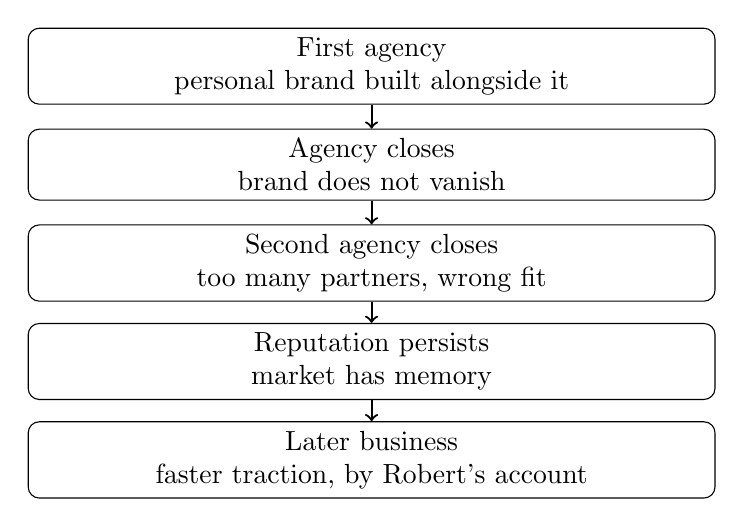
\begin{tikzpicture}[
  box/.style={draw, rounded corners, align=center, text width=0.70\linewidth, minimum height=0.55cm},
  arr/.style={->, thick}
]
\node[box] (a1) at (0,0) {First agency\\personal brand built alongside it};
\node[box] (a2) at (0,-1.25) {Agency closes\\brand does not vanish};
\node[box] (a3) at (0,-2.50) {Second agency closes\\too many partners, wrong fit};
\node[box] (a4) at (0,-3.75) {Reputation persists\\market has memory};
\node[box] (a5) at (0,-5.00) {Later business\\faster traction, by Robert's account};
\draw[arr] (a1) -- (a2);
\draw[arr] (a2) -- (a3);
\draw[arr] (a3) -- (a4);
\draw[arr] (a4) -- (a5);
\end{tikzpicture}
\end{figure}

\subsection{Question \& Answer}

\paragraph{Question.} What survived when the companies did not?

\paragraph{Answer.} Robert's answer is reputation: the personal brand, the trust, the accumulated market attention, and the proof that he could acquire clients and do digital marketing. In his telling, that durable asset helped him scale a later business to multiple seven figures in about six months and helped another reach a seven-figure runway within about sixty days.

\section{Partners, Failure, and Captive Risk}

The failure section begins with a constraint: Robert says that one only needs about two to three people in a partnership or company, not four to five. We should not make this a universal law, but we can preserve it as his operating rule:

\begin{equation}
n_{\mathrm{partners}} \approx 2\hbox{--}3,
\qquad
n_{\mathrm{partners}} = 4\hbox{--}5 \quad \hbox{is risky in this account.}
\end{equation}

The deeper point is not just headcount. It is execution and control. A name means little without execution. An offer means little without execution. A person can think the idea is valuable because he came up with it, but Robert pushes the value toward the people who actually carry out the work.

\begin{figure}
\centering
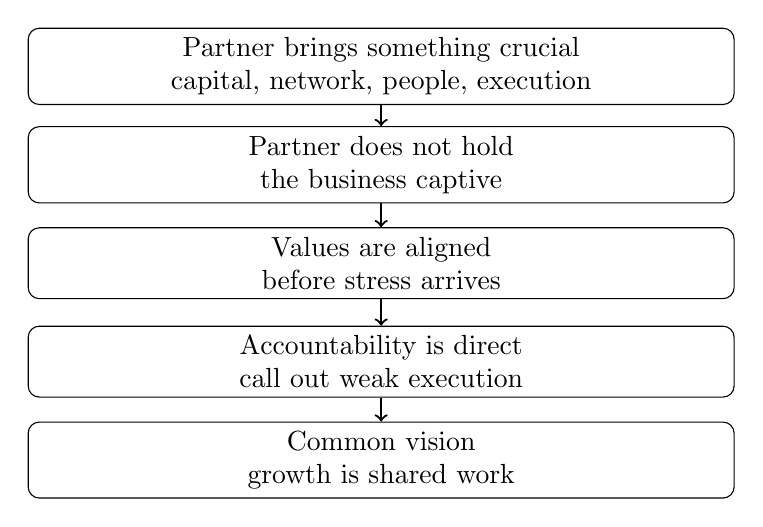
\begin{tikzpicture}[
  box/.style={draw, rounded corners, align=center, text width=0.72\linewidth, minimum height=0.55cm},
  arr/.style={->, thick}
]
\node[box] (p1) at (0,0) {Partner brings something crucial\\capital, network, people, execution};
\node[box] (p2) at (0,-1.25) {Partner does not hold\\the business captive};
\node[box] (p3) at (0,-2.50) {Values are aligned\\before stress arrives};
\node[box] (p4) at (0,-3.75) {Accountability is direct\\call out weak execution};
\node[box] (p5) at (0,-5.00) {Common vision\\growth is shared work};
\draw[arr] (p1) -- (p2);
\draw[arr] (p2) -- (p3);
\draw[arr] (p3) -- (p4);
\draw[arr] (p4) -- (p5);
\end{tikzpicture}
\end{figure}

There is an important emotional transition here. Robert speaks about loyalty and about not being able to do everything by himself. The lesson is not to avoid partners. It is to choose partners who are both useful and non-capturing: important to the function of the business, but not able to freeze it.

\section{Crypto, Energy, and the Question of Value}

The cryptocurrency section broadens the interview from business practice to monetary judgment. Robert says crypto is bigger than people think because it is not merely new technology; it is a new way to think about money. He brings in central banks, CBDCs, storage of wealth, scarcity, and cost.

The key question is whether value is just rarity, or whether society also attaches value to cost. In Robert's Bitcoin example, mining requires facilities, machines, electricity, and transaction verification. In the gold example, a bar also has to be mined. A compact representation of the analogy is:

\begin{align}
\hbox{Bitcoin verification} &\longleftarrow \hbox{machines} + \hbox{electricity} + \hbox{mining facility}, \\
\hbox{gold bar} &\longleftarrow \hbox{mining} + \hbox{energy} + \hbox{extraction cost}.
\end{align}

This is not a theorem of value. It is Robert's valuation intuition: we may value energy going into something that has scarce value. The open question is then whether society transacts with such a thing, stores wealth in it, or merely holds it as a scarce reserve.

\subsection{Question \& Answer}

\paragraph{Question.} Is value only rarity, or does cost matter?

\paragraph{Answer.} Robert argues that cost matters, at least as part of the story. He contrasts mere rarity with the physical cost of Bitcoin mining and the energy cost of obtaining a gold bar. The final notes should keep this as his claim, not as settled monetary theory: scarcity, verification, and energy cost are presented as reasons people may treat an asset as valuable.

\section{Breaks, Bad Debt, and Self-Investment}

The next turn asks what got Robert into crypto. The story becomes numerical. Around 2015--2016, in Simi Valley, he and his brother encountered someone deeply interested in the dark web and early digital coins. Robert recalls seeing references to 1,500 Bitcoins, later 15,000 Bitcoins, and eventually about 150,000 Bitcoins moving through a wallet address. When Bitcoin reached around a thousand dollars, the lesson became visible.

He says he got into Bitcoin around \( \$800 \) to \( \$1{,}000 \), Ethereum around \( \$17 \), and that AntShares, which converted into Neo, was a major project for him. His own small stake is the most concrete numerical example:

\begin{equation}
\$1{,}500\hbox{--}\$2{,}000
\longrightarrow
\sim \$250{,}000
\quad \hbox{in roughly four months.}
\end{equation}

The implied multiple is large:

\begin{align}
\frac{250{,}000}{2{,}000} &\approx 125, \\
\frac{250{,}000}{1{,}500} &\approx 167.
\end{align}

Those numbers should stay approximate. The transcript itself is approximate. The point is not precision; the point is that a small amount of capital became his first major financial break, and the break created a new social role. He began sharing information, creating books and courses, giving material away for free, and speaking about crypto.

The worst financial decision comes later: during payment-processor holds and what he calls an implosion in payment processing, he took out a flash loan for payroll coverage. He says the loan was paid off in about a month, so the lasting problem was not merely the debt. The loan exposed who was committed to the company and who was not.

The best financial decision is the inverse. After making money in crypto, he invested the rest into courses. He gives the range:

\begin{equation}
I_{\mathrm{edu}} \approx \$30{,}000\hbox{--}\$40{,}000.
\end{equation}

\paragraph{Worked example: the education bet.}
The mechanism can be written as an update rule for skill capital \(S\):

\begin{equation}
S_{t+1} = S_t + \Delta S(I_{\mathrm{edu}},M,E),
\end{equation}

where \(I_{\mathrm{edu}}\) is money spent on education, \(M\) is mentorship or mastermind exposure, and \(E\) is execution after learning. The return is not automatic. The update only matters if the learned skill is put back into the business.

In Robert's language, the purpose is to condense time. He learns stocks, e-commerce, and marketing, not to become an expert in everything, but to become more versatile and better able to choose his primary lane. Later, as the business gains traction, he invests in more mentorship. He gives an illustrative jump: a last mastermind may be the catalyst that helps a business go from one million dollars to seven million dollars in revenue, even though all the earlier learning set up the final connection.

\section{What Money Is For}

The last movement leaves mechanics and comes back to purpose. The greatest lesson, Robert says, is that relationships matter, but the right relationships matter most. The test is concrete: if there were only three numbers to dial in a life-or-death situation, who would be there?

Health becomes the next concrete lesson. Robert describes going the full burnout route, working sixteen-hour days, doing school and full-time work, operating from about 4 a.m. to midnight, and pulling an overnight effort for a government project. The point is not heroic labor. The point is the cost of ignoring the body.

The final question asks about long-term goals and motivation. Robert starts with the why. He describes growing up with a mother making roughly \( \$30{,}000 \) to \( \$40{,}000 \) a year in the suburbs of Los Angeles, and lacking food at times. That initial why was basic provision. Later, once food was no longer the issue, the why evolved: potential, impact, presence, becoming more than only the business person, and being able to help family. The example is direct: sending money to his mother when she needed help.

\section{Summary}

The interview's structure is a movement from windfall to operating discipline. Crypto creates capital, but capital gains are not cashflow. Business scale comes from attention, sales, and financial understanding. Personal brand survives failed vehicles and can carry trust into later ventures. Partners amplify the business only when they bring real function without holding the company captive. Crypto raises the larger question of how society assigns value to rarity, verification, and energy cost. The closing lesson is that money is not simply an accumulation target: it is a tool for education, time compression, relationships, health, family support, and the evolving why behind the work.